\documentclass[twoside]{book}

% Packages required by doxygen
\usepackage{fixltx2e}
\usepackage{calc}
\usepackage{doxygen}
\usepackage[export]{adjustbox} % also loads graphicx
\usepackage{graphicx}
\usepackage[utf8]{inputenc}
\usepackage{makeidx}
\usepackage{multicol}
\usepackage{multirow}
\PassOptionsToPackage{warn}{textcomp}
\usepackage{textcomp}
\usepackage[nointegrals]{wasysym}
\usepackage[table]{xcolor}

% Font selection
\usepackage[T1]{fontenc}
\usepackage[scaled=.90]{helvet}
\usepackage{courier}
\usepackage{amssymb}
\usepackage{sectsty}
\renewcommand{\familydefault}{\sfdefault}
\allsectionsfont{%
  \fontseries{bc}\selectfont%
  \color{darkgray}%
}
\renewcommand{\DoxyLabelFont}{%
  \fontseries{bc}\selectfont%
  \color{darkgray}%
}
\newcommand{\+}{\discretionary{\mbox{\scriptsize$\hookleftarrow$}}{}{}}

% Page & text layout
\usepackage{geometry}
\geometry{%
  a4paper,%
  top=2.5cm,%
  bottom=2.5cm,%
  left=2.5cm,%
  right=2.5cm%
}
\tolerance=750
\hfuzz=15pt
\hbadness=750
\setlength{\emergencystretch}{15pt}
\setlength{\parindent}{0cm}
\setlength{\parskip}{3ex plus 2ex minus 2ex}
\makeatletter
\renewcommand{\paragraph}{%
  \@startsection{paragraph}{4}{0ex}{-1.0ex}{1.0ex}{%
    \normalfont\normalsize\bfseries\SS@parafont%
  }%
}
\renewcommand{\subparagraph}{%
  \@startsection{subparagraph}{5}{0ex}{-1.0ex}{1.0ex}{%
    \normalfont\normalsize\bfseries\SS@subparafont%
  }%
}
\makeatother

% Headers & footers
\usepackage{fancyhdr}
\pagestyle{fancyplain}
\fancyhead[LE]{\fancyplain{}{\bfseries\thepage}}
\fancyhead[CE]{\fancyplain{}{}}
\fancyhead[RE]{\fancyplain{}{\bfseries\leftmark}}
\fancyhead[LO]{\fancyplain{}{\bfseries\rightmark}}
\fancyhead[CO]{\fancyplain{}{}}
\fancyhead[RO]{\fancyplain{}{\bfseries\thepage}}
\fancyfoot[LE]{\fancyplain{}{}}
\fancyfoot[CE]{\fancyplain{}{}}
\fancyfoot[RE]{\fancyplain{}{\bfseries\scriptsize Generated by Doxygen }}
\fancyfoot[LO]{\fancyplain{}{\bfseries\scriptsize Generated by Doxygen }}
\fancyfoot[CO]{\fancyplain{}{}}
\fancyfoot[RO]{\fancyplain{}{}}
\renewcommand{\footrulewidth}{0.4pt}
\renewcommand{\chaptermark}[1]{%
  \markboth{#1}{}%
}
\renewcommand{\sectionmark}[1]{%
  \markright{\thesection\ #1}%
}

% Indices & bibliography
\usepackage{natbib}
\usepackage[titles]{tocloft}
\setcounter{tocdepth}{3}
\setcounter{secnumdepth}{5}
\makeindex

% Hyperlinks (required, but should be loaded last)
\usepackage{ifpdf}
\ifpdf
  \usepackage[pdftex,pagebackref=true]{hyperref}
\else
  \usepackage[ps2pdf,pagebackref=true]{hyperref}
\fi
\hypersetup{%
  colorlinks=true,%
  linkcolor=blue,%
  citecolor=blue,%
  unicode%
}

% Custom commands
\newcommand{\clearemptydoublepage}{%
  \newpage{\pagestyle{empty}\cleardoublepage}%
}

\usepackage{caption}
\captionsetup{labelsep=space,justification=centering,font={bf},singlelinecheck=off,skip=4pt,position=top}

%===== C O N T E N T S =====

\begin{document}

% Titlepage & ToC
\hypersetup{pageanchor=false,
             bookmarksnumbered=true,
             pdfencoding=unicode
            }
\pagenumbering{alph}
\begin{titlepage}
\vspace*{7cm}
\begin{center}%
{\Large simulation.\+h }\\
\vspace*{1cm}
{\large Generated by Doxygen 1.8.13}\\
\end{center}
\end{titlepage}
\clearemptydoublepage
\pagenumbering{roman}
\tableofcontents
\clearemptydoublepage
\pagenumbering{arabic}
\hypersetup{pageanchor=true}

%--- Begin generated contents ---
\chapter{File Index}
\section{File List}
Here is a list of all documented files with brief descriptions\+:\begin{DoxyCompactList}
\item\contentsline{section}{include/\hyperlink{car_8h}{car.\+h} \\*File containing the function definitions needed for car struct }{\pageref{car_8h}}{}
\end{DoxyCompactList}

\chapter{File Documentation}
\hypertarget{simulation_8h}{}\section{include/simulation.h File Reference}
\label{simulation_8h}\index{include/simulation.\+h@{include/simulation.\+h}}


File containing the function definitions needed for the simulation.  


{\ttfamily \#include $<$stdio.\+h$>$}\newline
{\ttfamily \#include $<$stdlib.\+h$>$}\newline
Include dependency graph for simulation.\+h\+:
\nopagebreak
\begin{figure}[H]
\begin{center}
\leavevmode
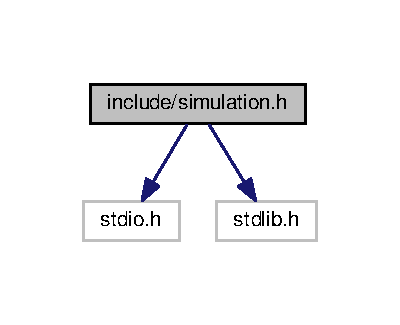
\includegraphics[width=192pt]{simulation_8h__incl}
\end{center}
\end{figure}
\subsection*{Functions}
\begin{DoxyCompactItemize}
\item 
void \hyperlink{simulation_8h_a90e2cfe51ee0acd70b990bda1c194abb}{add\+Car\+To\+Queues} (Queue $\ast$all\+Queue\mbox{[}$\,$\mbox{]}, Queue $\ast$all\+Cars)
\item 
void \hyperlink{simulation_8h_a06f1e3f509e31f4c54a779dcf3281b23}{updateintersection\+Queue} (Queue $\ast$all\+Queue\mbox{[}$\,$\mbox{]}, Queue $\ast$intersection\+Queue, double wait\+Timer, char wait\+Car)
\item 
Car $\ast$ \hyperlink{simulation_8h_a9a741f449eda8902f99b90f08baaf1d4}{remove\+Car\+From\+Queues} (Queue $\ast$all\+Queue\mbox{[}$\,$\mbox{]}, Queue $\ast$intersection\+Queue)
\item 
void \hyperlink{simulation_8h_a8966dfbadef886108cf48deba0ec2dab}{update\+Waiting\+Time} (Queue $\ast$all\+Queue\mbox{[}$\,$\mbox{]})
\item 
void \hyperlink{simulation_8h_af4bdd480490de76f701f2f39550783d8}{report\+Max\+Waiting\+Time} (Queue $\ast$order)
\item 
void \hyperlink{simulation_8h_a649d4ab7de85af7209a00d4198ca6320}{report\+Average\+Waiting\+Time} (Queue $\ast$order, Queue $\ast$all\+Queue\mbox{[}$\,$\mbox{]})
\end{DoxyCompactItemize}


\subsection{Detailed Description}
File containing the function definitions needed for the simulation. 

\begin{DoxyAuthor}{Author}
Ralph Arvin De Castro 
\end{DoxyAuthor}
\begin{DoxyDate}{Date}
June 2018 
\end{DoxyDate}


\subsection{Function Documentation}
\mbox{\Hypertarget{simulation_8h_a90e2cfe51ee0acd70b990bda1c194abb}\label{simulation_8h_a90e2cfe51ee0acd70b990bda1c194abb}} 
\index{simulation.\+h@{simulation.\+h}!add\+Car\+To\+Queues@{add\+Car\+To\+Queues}}
\index{add\+Car\+To\+Queues@{add\+Car\+To\+Queues}!simulation.\+h@{simulation.\+h}}
\subsubsection{\texorpdfstring{add\+Car\+To\+Queues()}{addCarToQueues()}}
{\footnotesize\ttfamily void add\+Car\+To\+Queues (\begin{DoxyParamCaption}\item[{Queue $\ast$}]{all\+Queue\mbox{[}$\,$\mbox{]},  }\item[{Queue $\ast$}]{all\+Cars }\end{DoxyParamCaption})}

Adds car to their respective queues 
\begin{DoxyParams}{Parameters}
{\em all\+Queue} & double pointer of queue N S E W \\
\hline
{\em all\+Cars} & pointer queue of all cars \\
\hline
\end{DoxyParams}
\mbox{\Hypertarget{simulation_8h_a9a741f449eda8902f99b90f08baaf1d4}\label{simulation_8h_a9a741f449eda8902f99b90f08baaf1d4}} 
\index{simulation.\+h@{simulation.\+h}!remove\+Car\+From\+Queues@{remove\+Car\+From\+Queues}}
\index{remove\+Car\+From\+Queues@{remove\+Car\+From\+Queues}!simulation.\+h@{simulation.\+h}}
\subsubsection{\texorpdfstring{remove\+Car\+From\+Queues()}{removeCarFromQueues()}}
{\footnotesize\ttfamily Car$\ast$ remove\+Car\+From\+Queues (\begin{DoxyParamCaption}\item[{Queue $\ast$}]{all\+Queue\mbox{[}$\,$\mbox{]},  }\item[{Queue $\ast$}]{intersection\+Queue }\end{DoxyParamCaption})}

remove car from queues once it goes through the intersection \begin{DoxyReturn}{Returns}
pointer to the car that is removed 
\end{DoxyReturn}

\begin{DoxyParams}{Parameters}
{\em all\+Queue} & double pointer of queue N S E W \\
\hline
{\em intersection\+Queue} & pointer of queue that has the wait list \\
\hline
\end{DoxyParams}
\mbox{\Hypertarget{simulation_8h_a649d4ab7de85af7209a00d4198ca6320}\label{simulation_8h_a649d4ab7de85af7209a00d4198ca6320}} 
\index{simulation.\+h@{simulation.\+h}!report\+Average\+Waiting\+Time@{report\+Average\+Waiting\+Time}}
\index{report\+Average\+Waiting\+Time@{report\+Average\+Waiting\+Time}!simulation.\+h@{simulation.\+h}}
\subsubsection{\texorpdfstring{report\+Average\+Waiting\+Time()}{reportAverageWaitingTime()}}
{\footnotesize\ttfamily void report\+Average\+Waiting\+Time (\begin{DoxyParamCaption}\item[{Queue $\ast$}]{order,  }\item[{Queue $\ast$}]{all\+Queue\mbox{[}$\,$\mbox{]} }\end{DoxyParamCaption})}

Calculate and print average waiting times 
\begin{DoxyParams}{Parameters}
{\em order} & pointer to a queue that has the order of the cars going through the intersection \\
\hline
{\em all\+Queue} & double pointer of queue N S E W \\
\hline
\end{DoxyParams}
\mbox{\Hypertarget{simulation_8h_af4bdd480490de76f701f2f39550783d8}\label{simulation_8h_af4bdd480490de76f701f2f39550783d8}} 
\index{simulation.\+h@{simulation.\+h}!report\+Max\+Waiting\+Time@{report\+Max\+Waiting\+Time}}
\index{report\+Max\+Waiting\+Time@{report\+Max\+Waiting\+Time}!simulation.\+h@{simulation.\+h}}
\subsubsection{\texorpdfstring{report\+Max\+Waiting\+Time()}{reportMaxWaitingTime()}}
{\footnotesize\ttfamily void report\+Max\+Waiting\+Time (\begin{DoxyParamCaption}\item[{Queue $\ast$}]{order }\end{DoxyParamCaption})}

Calculate and print maximum waiting time 
\begin{DoxyParams}{Parameters}
{\em order} & pointer to a queue that has the order of the cars going through the intersection \\
\hline
\end{DoxyParams}
\mbox{\Hypertarget{simulation_8h_a06f1e3f509e31f4c54a779dcf3281b23}\label{simulation_8h_a06f1e3f509e31f4c54a779dcf3281b23}} 
\index{simulation.\+h@{simulation.\+h}!updateintersection\+Queue@{updateintersection\+Queue}}
\index{updateintersection\+Queue@{updateintersection\+Queue}!simulation.\+h@{simulation.\+h}}
\subsubsection{\texorpdfstring{updateintersection\+Queue()}{updateintersectionQueue()}}
{\footnotesize\ttfamily void updateintersection\+Queue (\begin{DoxyParamCaption}\item[{Queue $\ast$}]{all\+Queue\mbox{[}$\,$\mbox{]},  }\item[{Queue $\ast$}]{intersection\+Queue,  }\item[{double}]{wait\+Timer,  }\item[{char}]{wait\+Car }\end{DoxyParamCaption})}

Updates intersection queue or the wait list for the intersection 
\begin{DoxyParams}{Parameters}
{\em all\+Queue} & double pointer of queue N S E W \\
\hline
{\em intersection\+Queue} & pointer of queue that has the wait list \\
\hline
{\em wait\+Timer} & timer that determines if a car can move to the front of the queue \\
\hline
{\em wait\+Car} & the car that must wait \\
\hline
\end{DoxyParams}
\mbox{\Hypertarget{simulation_8h_a8966dfbadef886108cf48deba0ec2dab}\label{simulation_8h_a8966dfbadef886108cf48deba0ec2dab}} 
\index{simulation.\+h@{simulation.\+h}!update\+Waiting\+Time@{update\+Waiting\+Time}}
\index{update\+Waiting\+Time@{update\+Waiting\+Time}!simulation.\+h@{simulation.\+h}}
\subsubsection{\texorpdfstring{update\+Waiting\+Time()}{updateWaitingTime()}}
{\footnotesize\ttfamily void update\+Waiting\+Time (\begin{DoxyParamCaption}\item[{Queue $\ast$}]{all\+Queue\mbox{[}$\,$\mbox{]} }\end{DoxyParamCaption})}

Updates waiting time of each car in the queue 
\begin{DoxyParams}{Parameters}
{\em all\+Queue} & double pointer of queue N S E W \\
\hline
\end{DoxyParams}

%--- End generated contents ---

% Index
\backmatter
\newpage
\phantomsection
\clearemptydoublepage
\addcontentsline{toc}{chapter}{Index}
\printindex

\end{document}
